\subsection{Die Wellenlängen der Spektrallinien}
Für Berechnungen werden die genauen Wellenlängen der Spektrallinien benötigt. Um sie zu bestimmen wird ein Auszug aus \cite[Tabellenanhang Tab. A 4.3]{Walcher} (Tablle \ref{tab:Wellenlange}) verwendet. Bei der Messung wird ein Spektrum wie in Abbildung \ref{abb:Spektrum}, allerdings ohne die kurzwelligen dunkelroten Linien, gesehen.
\begin{table}[h!]
	\centering
	\begin{tabular}{llll}
		Element & $\lambda$ in \si{\nano\meter} & Farbeindruck & Helligkeitseindruck\footnotemark \\
		\hline
		Cadmium (Cd) & 643.86 & rot & stark \\
		& 635.99 & gelbrot & schwach \\
		& 508.58 & grün & stark \\
		& 479.99 & blaugrün & stark \\
		& 467.82 & blau & stark \\
		& 441.46 & blau & mittel \\
		\hline
		Quecksilber (Hg) & 708.19 & rot & schwach \\
		& 690.72 & rot & schwach \\
		& 579.07 & gelb & sehr stark \\
		& 576.96 & gelb & sehr stark \\
		& 546.07 & grün & stark \\
		& 491.60 & blaugrün & mittel \\
		& 435.84 & blau & stark \\
		& 407.78 & violett & mittel \\
		& 404.66 & violett & mittel \\
		\hline
	\end{tabular}
	\caption{Wellenlängen der Spektrallinien von Cadmium und Quecksilber}
	\label{tab:Wellenlange}
\end{table}
\footnotetext{relative Lichtstärke für ein einzelnes Element}
\begin{figure}[h!]
	\centering
	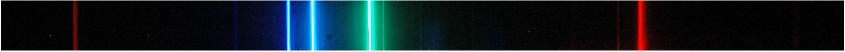
\includegraphics[width = \textwidth]{Cd.jpg}
	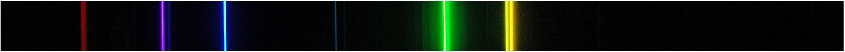
\includegraphics[width = \textwidth]{Hg.jpg}
	\caption{Spektrallinien einer Cadmiumspektrallampe\cite{Cadmium} (oben) und einer Quecksilberdampflampe\cite{Quecksilber} (unten)}
	\label{abb:Spektrum}
\end{figure}\newline
Durch Kombination von Tabelle \ref{tab:Wellenlange} und Abbildung \ref{abb:Spektrum} wird sich für die in Tabelle \ref{tab:Wellen} aufgelisteten Wellenlängen entschieden.
\begin{table}[h!]
\centering
\begin{tabular}{lll}
	Farbe & $\lambda$ in \si{\nano\meter} & Element \\
	\hline
	rot & 643.86 & Cd \\
	gelb & 576.96 / 579.07 & Hg \\
	grün & 546.07 & Hg \\
	grün & 508.58 & Cd \\
	blaugrün & 479.99 & Cd \\
	blau & 467.82 & Cd \\
	blau & 435.84 / 441.46 & Hg / Cd \\
	violett & 404.66 / 407.78 & Hg
\end{tabular}
\caption{Beobachtete Wellenlängen}
\label{tab:Wellen}
\end{table}
\clearpage


\subsection{Berechnung von Innenwinkel und Brechwinkel}
Bei der Messung des Innenwinkels des Prismas und mit Formel \eqref{Phi} ergeben sich die die Werte in Tabelle \ref{tab:WinkelPhi}. Der Mittelwert\footnote{siehe \ref{math:ErrorAver}} ist
\begin{align}
	\overline{\varphi} = \SI{54.8+-0.3}{}
 \ .
\end{align}
\begin{table}[h!]
	\centering	
	\begin{tabular}{c|c|c}
		$\varphi_r$ & $\varphi_l$ & $\varphi$ \\
		\hline
		376.0 & 266.0 & 55.0 \\
376.0 & 265.5 & 55.2 \\
376.0 & 265.7 & 55.2 \\

	\end{tabular}
	\caption{Messwerte zur Bestimmung des Innenwinkels $\varphi$ in \si{\degree}}
	\label{tab:WinkelPhi}
\end{table} \\
Die nachfolgenden Werte werden allerdings mit dem zu erwartenden Wert $\varphi= \SI{60}{\degree}$ berechnet.
Tabelle \ref{tab:WinkelFarben} zeigt die Winkel $\Omega_l$ und $\Omega_r$, die zusammen mit Formel \eqref{Eta} die Werte für die Brechwinkel $\eta$ ergeben.
\begin{table}[h!]
	\centering	
	\begin{tabular}{c|c|c|c}
		Wellenlänge $\lambda$ in \si{\nano\meter} & $\Omega_l$ & $\Omega_r$ & $\eta$ \\
		\hline
		406.22 & 11.4 & 252.1 & 60.7 \\
438.65 & 12.1 & 252.0 & 59.9 \\
467.82 & 13.1 & 252.9 & 59.8 \\
479.99 & 8.7  & 254.6 & 65.9 \\
508.58 & 14.1 & 254.6 & 60.5 \\
546.07 & 14.6 & 255.1 & 60.5 \\
578.02 & 15.0 & 255.5 & 60.5 \\
643.86 & 11.2 & 255.9 & 64.7 \\

	\end{tabular}
	\caption{Messwerte zur Bestimmung des Brechwinkels $\eta$ in \si{\degree}}
	\label{tab:WinkelFarben}
\end{table}
\clearpage


\subsection{Bestimmung der Dispersionskurve}
Mit Hilfe von Formel \eqref{BrechIndex} kann nun für jede Wellenlänge $\lambda$ der Brechungsindex (siehe Tabelle \ref{tab:Brechzahl}) ausgerechnet werden.
\begin{table}[h!]
	\centering	
	\begin{tabular}{c|c|c}
		$\lambda$ in \si{\nano\meter} & $n$ & Fehler $\Delta_n$ \\
		\hline
		406.22 & 1.965 & 0.000 \\
438.65 & 1.959 & 0.000 \\
467.82 & 1.957 & 0.000 \\
479.99 & 1.950 & 0.000 \\
508.58 & 1.947 & 0.000 \\
546.07 & 1.941 & 0.000 \\
578.02 & 1.935 & 0.000 \\
643.86 & 1.919 & 0.000 \\

	\end{tabular}
	\caption[Errechnete Brechzahlen $n$ mit Fehlern für jede Wellenlänge $\lambda$]{Errechnete Brechzahlen $n$ mit Fehlern\footnotemark\ für jede Wellenlänge $\lambda$}
	\label{tab:Brechzahl}
\end{table}
\footnotetext{siehe: \ref{math:ErrorBrechindex}} \\
Wie in der Theorie beschrieben muss nun entschieden werden, ob das betrachtete Spektrum über (Fall 1) oder unter (Fall 2) der Absorptionsstelle liegt. Dazu werden Formel \eqref{Fall1} als
\begin{align}\label{Reg:1}
	n^2(\lambda) = A_0 + \frac{A_2}{\lambda^2}
\end{align}
und Formel \eqref{Fall2} als
\begin{align}\label{Reg:2}
	n^2(\lambda) = A_0' + A_2'\lambda^2
\end{align}
genähert. Es wird jeweils eine lineare Regression\footnote{siehe: \ref{math:Regression}} mit den Wertepaaren $\{ (\frac{1}{\lambda_i^2}, n^2(\lambda_i)) \}$ (bei \eqref{Reg:1}) bzw. $\{ (\lambda_i^2, n^2(\lambda_i)) \}$ (bei \eqref{Reg:2}) durchgeführt, um die Parameter $A_0, A_2, A_0', A_2'$ auszurechnen. Die \glqq Güte\grqq\ der Parameter kann durch die quadratischen Abweichungen\footnote{siehe: \ref{math:QuadrAbw}} $s^2, s'^2$ bestimmt werden. Alle diese Werte finden sich in Tabelle \ref{tab:Regression}.
\begin{table}[h!]
	\centering
	\begin{tabular}{c|c|c}
		Größe & Wert & relativer Fehler \\
		\hline
		$A_2$ & \SI{4.6+-0.6e-14}{\meter\squared}
 & \SI{-0.1}{\meter\squared}
 \\
		$A_2'$ & \SI{-7.0+-0.2e-25}{\meter^{-2}}
 & \SI{-0.0}{\meter^{-2}}
 \\
		$A_0$ & \SI{3.60+-0.02}{}
 & \SI{0.007}{}
 \\
		$A_0'$ & \SI{3.974+-0.006}{}
 & \SI{0.002}{}
 \\
		\hline
		$s^2(A_0,A_2)$ & \SI{0.3e-3}{}
 & \\
		$s'^2(A_0',A_2')$ & \SI{49.2e-3}{}
 &
	\end{tabular}
	\caption{Durch die lineare Regression berechnete Werte $A_0,A_0',A_2,A_2'$ mit Fehlern und relativen Fehlern, sowie die quadratischen Abweichungen $s^2,s'^2$ der Regressionsgeraden zu den Datenpunkten}
	\label{tab:Regression}
\end{table}
Eigentlich sollte die Entscheidung welche Näherung die bessere ist, allein durch Betrachtung der Krümmung der Kurve, die die Messwerte in Abbildung \ref{Abb:Krummung} beschreiben, getroffen werden können. In diesem Fall ist das nicht sehr aussagekräftig, weshalb sich hier nur auf die Abweichungsquadrate verlassen wird. Demnach ist \eqref{Reg:1} die bessere Wahl und die Dispersionsgleichung wird zu
\begin{align*}
	n(\lambda) = \sqrt{3.6 + \SI{4.6e-14}\lambda^{-2}}
\end{align*}
bestimmt. Der Funktionsgraf ist in Abbildung \ref{fig:DispKurve} zu sehen.
\begin{figure}[h!]
	\centering
	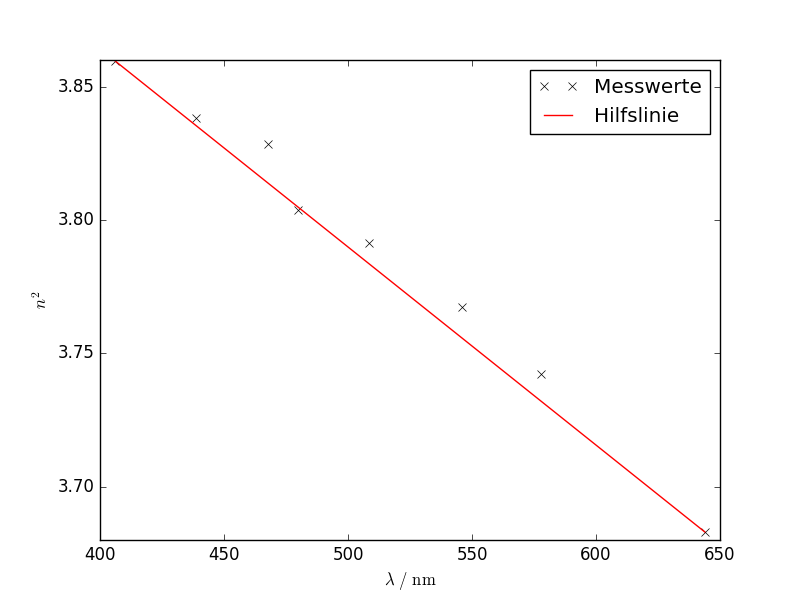
\includegraphics[width=0.7\textwidth]{Tendenz.png}
	\caption{Graphik zur Abschätzung, ob die Absorptionsstelle größer oder kleiner als das betrachtete Spektrum ist}
	\label{Abb:Krummung}
\end{figure}
\begin{figure}[h!]
	\centering
	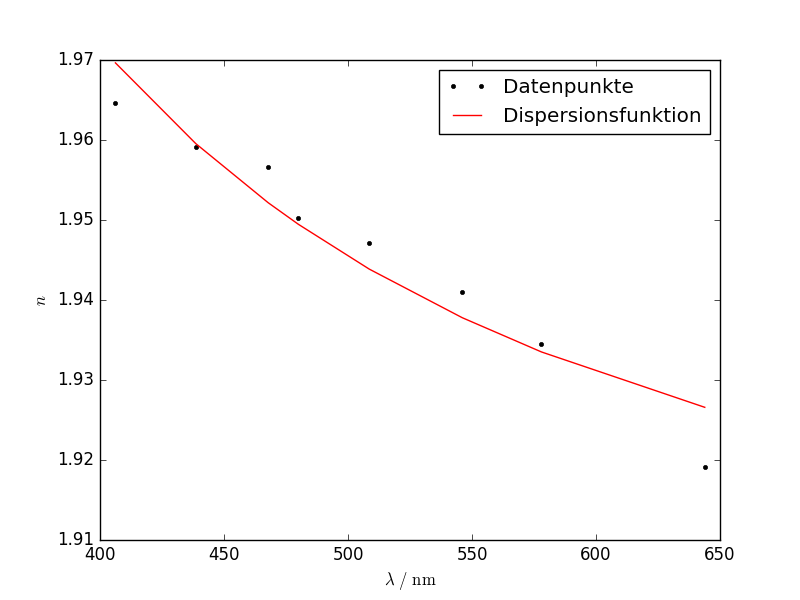
\includegraphics[width=0.7\textwidth]{Dispersionskurve.png}
	\caption{Dispersionskurve}
	\label{fig:DispKurve}
\end{figure}
\newline
Für die nächstgelegene Absorptionsstelle $\lambda_1$ gilt also $\lambda_1\gg\lambda_i$. Es wird davon ausgegangen, dass es nur eine Absorptionsstelle gibt. Es folgt dann aus \eqref{Absorptionsstelle}, dass der Brechindex für $\omega\rightarrow\omega_1$ bzw. $\lambda\rightarrow\lambda_1$ gegen 1 geht. Es gilt für \eqref{Reg:1}:
\begin{align*}
	n^2(\lambda_1) = 1 &= A_0 + \frac{A_2}{\lambda_1^2} \\
	\Leftrightarrow\quad \lambda_1 &= \sqrt{\frac{A_2}{A_0-1}} = \SI{9.664e-8}{\nano\meter}
 \ .
\end{align*}
\clearpage
\subsection{Kenndaten des Prismas\label{sec:Kenndaten}}
Zuletzt sollen einige Kenndaten des verwendeten Prismas berechnet werden. \\
\ \\
Die Abbesche Zahl ist ein Maß für die Farbzerstreuung bei Gläsern. Sie ist definiert als
\begin{align}
	\nu = \frac{n_\text{D}-1}{n_\text{F}-n_\text{C}} \ ,
\end{align}
wobei die $n_\text{I}$ die Brechzahlen der Fraunhoferschen Linien $\lambda_\text{D} = \SI{589}{\nano\meter}$, $\lambda_\text{F} = \SI{486}{\nano\meter}$ und $\lambda_\text{C} = \SI{656}{\nano\meter}$ sind. Sie hat hier den Wert
\begin{align}
	\nu = \SI{-70.789}{}
 \ .
\end{align}
\ \\
Das Auflösungsvermögen bezeichnet den Koeffizienten $\frac{\lambda}{\Delta\lambda}$, der beschreibt, wie nah zwei Spektrallinien liegen dürfen, sodass sie vom Prisma noch getrennt werden können. Für das verwendete Prisma kann das Auflösungsvermögen mit
\begin{align*}
	\left|\frac{\lambda}{\Delta\lambda}\right| = \left|b\frac{\text{d}n}{\text{d}\lambda}\right| = b\frac{\SI{4.6e-14}\lambda^{-3}}{\sqrt{3.6+\SI{4.6e-14}\lambda^{-2}}}
\end{align*}
berechnet werden (Werte für jede Wellenlänge siehe Tabelle \ref{tab:Aufl}). Die Länge $b=\SI{3}{\centi\meter}$ ist die Seitenlänge des Prismas.
\begin{table}[h!]
	\centering
	\begin{tabular}{c|c}
		Wellenlänge in \si{\nano\meter} & Auflösungsvermögen \\
		\hline
		406.2 & 10449 \\
438.7 & 8341  \\
467.8 & 6902  \\
480.0 & 6399  \\
508.6 & 5395  \\
546.1 & 4372  \\
578.0 & 3695  \\
643.9 & 2683  \\

	\end{tabular}
	\caption{Auflösungsvermögen bei verschiedenen Wellenlängen}
	\label{tab:Aufl}
\end{table}

